\documentclass[aspectratio=169]{beamer}
\usepackage{beamerstyle}

\begin{document}

% Title slide
\begin{frame}
	\vspace{2cm}
	\begin{center}
		{\Huge\textbf{\textcolor{copenhagenred}{Rejection Sampling}}}
		\vspace{1cm}

		\rule{4cm}{3pt}
		\vspace{2cm}
	\end{center}
\end{frame}


\begin{frame}{why}
	Basic idea: Sample from instrumental proposal $q \neq \pi$; correct
	through rejection step to obtain a sample from $\pi$.

	Given two densities $\pi,q$ with $\pi ( x ) \leq M q ( x )$ for all $x$, and some $M > 0$, we can generate a sample from $\pi$ by
\end{frame}

% Slide 1
\begin{frame}{What is Rejection Sampling?}
	\begin{columns}
		\column{0.5\textwidth}
		\textbf{Intuition:}
		\begin{itemize}
			\item Throw darts uniformly under $M \cdot q(x)$
			\item Keep only those under $\pi(x)$
			\item Kept points follow $\pi(x)$ exactly!
		\end{itemize}

		\vspace{0.2cm}
		\textbf{The Algorithm:}
		\begin{enumerate}
			\item Sample $X \sim q(x)$
			\item Sample $U \sim \text{Uniform}(0,1)$
			\item Accept if $U \leq \frac{\pi(X)}{M \cdot q(X)}$
		\end{enumerate}

		\vspace{0.2cm}
		\textbf{Why it works:} We're sampling uniformly from the area under $\pi(x)$!

		\column{0.5\textwidth}
		\begin{center}
			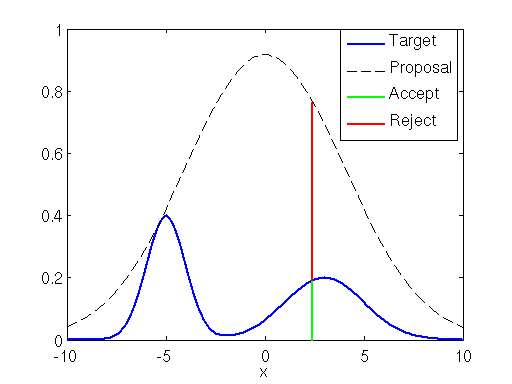
\includegraphics[width=0.95\textwidth]{rejectionsamplingcriterion.png}
		\end{center}

	\end{columns}
\end{frame}


% Slide 2
\begin{frame}{Mathematical Foundation}
	\begin{proposition}
		The distribution of accepted samples is exactly $\pi(x)$
	\end{proposition}
	\textbf{Proof:} We need to show $P(X \in A | X \text{ accepted}) = \pi(A)$. From the
	definition of conditional probability: $P(X \in A | X \text{ accepted}) = \frac{P(X \in A, X \text{ accepted})}{P(X \text{ accepted})}$.

	\begin{align*}
		P(X \in A, X \text{ accepted}) & = \int_X \int_0^1 \mathbb{I}_A(x) \cdot \mathbb{I}\left(u \leq \frac{\pi(x)}{M q(x)}\right) q(x) \, du \, dx \\
		                               & = \int_X \mathbb{I}_A(x) \cdot \frac{\pi(x)}{M q(x)} \cdot q(x) \, dx                                        \\
		                               & = \int_X \mathbb{I}_A(x) \cdot \frac{\pi(x)}{M} \, dx = \frac{\pi(A)}{M}
	\end{align*}

	Similarly, $P(X \text{ accepted}) = \frac{1}{M}$. Therefore: $P(X \in A | X \text{ accepted}) = \frac{\pi(A)/M}{1/M} = \pi(A)$.

\end{frame}

\begin{frame}{Does this work for un-normalised distributions?}
	Often we only know $\pi$ and $q$ up to some normalising constants; i.e.
	\begin{equation*}
		\pi = \frac{\pi}{Z_\pi} \quad \text{and} \quad q = \frac{q}{Z_q}
	\end{equation*}

	where $\tilde{\pi}$, $\tilde{q}$ are known but $Z_\pi$, $Z_q$ are unknown.
	You still need to be able to sample from $q(\cdot)$.
	If you can upper bound:
	\begin{equation*}
		\frac{\tilde{\pi}(x)}{\tilde{q}(x)} \leq \tilde{M},
	\end{equation*}
	then using $\tilde{\pi}$, $\tilde{q}$ and $\tilde{M}$ in the algorithm is correct.


	Indeed we have
	\begin{equation*}
		\frac{\tilde{\pi}(x)} {\tilde{q}(x)} \leq \tilde{M} \iff
		\frac{\pi(x)}{q(x)} \leq \tilde{M} \cdot \frac{Z_q}{Z_\pi} \overset{\text{def}}{=} M
	\end{equation*}

\end{frame}

\begin{frame}
	\begin{itemize}
		\item forudsætninger og konstant $M$
		\item waiting time to accepted sample is geometric with mean $M$
		\item $M$ storre end 1
		\item find $M$ kan være svært
		\item kan være ineffektiv hvis $M$ er stor
		\item dimensionalitet
		\item squeezing
	\end{itemize}
\end{frame}

\end{document}